\documentclass[tikz,border=4pt]{standalone}
\usepackage{amsmath,amssymb}

\usetikzlibrary{arrows.meta,positioning,automata,shapes,shapes.misc,calc,decorations.pathmorphing,decorations.markings,angles,quotes,patterns,mindmap,matrix,knots,hobby,trees}
\tikzset{->-/.style={decoration={markings, mark=at position 0.5 with {\arrow{Stealth}}}, postaction={decorate}}}
\begin{document}
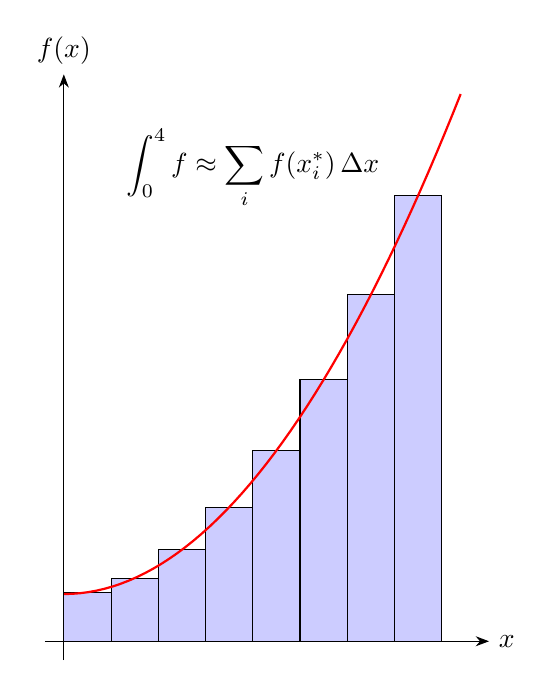
\begin{tikzpicture}[scale=1.2, >=Stealth]
\foreach \x in {0,0.5,...,3.5} \draw[fill=blue!20] (\x,0) rectangle (\x+0.5,{0.3*(\x+0.25)^2+0.5});
\draw[thick, red, domain=0:4.2, samples=50] plot (\x,{0.3*\x^2+0.5});
\draw[->] (-0.2,0) -- (4.5,0) node[right] {$x$}; \draw[->] (0,-0.2) -- (0,6) node[above] {$f(x)$};
\node at (2,5) {$\displaystyle\int_0^4 f \approx \sum_{i} f(x_i^*)\,\Delta x$};
\end{tikzpicture}
\end{document}
